\section{Ejercicio 1}

\subsection{Diseño del Circuito}

Se deseo diseñar un filtro notch pasivo con $f_0$ = $18.9 kHz$ para el siguiente circuito: 

\begin{figure}[h]
	\centering
	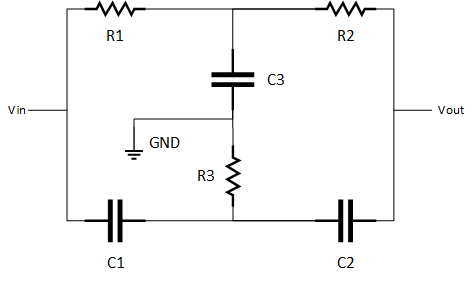
\includegraphics[scale=1]{../EJ1/circuito.png}
	\caption{Filtro Notch Pasivo}
	\label{ej1cir}
\end{figure}

La determinación de los valores de las resistencias y capacitores requieren primeramente la función de trasferencia del circuito, es decir que se deberá hallar una resolución del circuito. Para ello tomaremos las siguientes direcciones de corriente, de las cuales obtenemos las siguientes ecuaciones:

\begin{wrapfigure}{l}{0.5\textwidth}
\centering
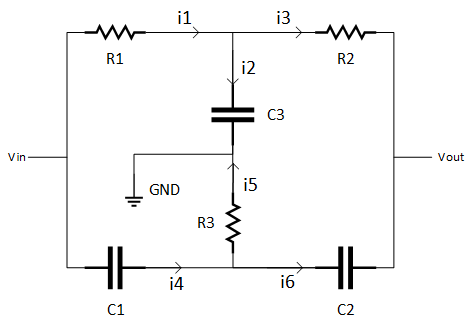
\includegraphics[scale=0.6]{../EJ1/circuitois.png}
\caption{Flujo de Corrientes}
\label{fig_2}
\end{wrapfigure}


$$Vin = R_1 *i_1 + X_{C3}.i_2 \hspace{1cm} Vout = -R_2 .i_3 + X_{C3}.i_2$$
$$Vin = R_3 .i_5 + X_{C2}.i_4 \hspace{1cm} Vout = R_3 .i_5 - X_{C2}.i_2$$

Como sabemos que $i_1 = i_2 + i_3$, $i_4 = i_5 + i_6$ y $i_6 = - i_3$ podemos analizar las ecuaciones algebraicamente resultando en:

$$i_2 (R_1 + 2.X_{C3}) = i_5 (2.R_3+X_{C1}) + i_3 (X_{C2} - X_{C1})$$\\


Al considerar $R = R1 = R2 = 2 \cdot R3$ y $C = C1 = C2 = \frac{C3}{2}$ 
$$\therefore i_2 = i_5$$

Por lo que la función de transferencia sera igual a:

$$\frac{Vout}{Vin} = \frac{X_C^2 + R^2}{R^2 + 4RX_c + X_C^2} \hspace{0.5cm}\Rightarrow \hspace{0.5cm} H(s) = \frac{s^2C^2R^2 + 1}{s^2R^2C^2 + s4RC + 1}$$

Pues entonces $$\omega_0 = \frac{1}{RC} \hspace{0.5cm} \Rightarrow \hspace{0.5cm} f_0 = \frac{1}{2\pi RC}$$. De acuerdo a esto y considerando que solo tenemos resistencias y capacitores comerciables, para que $f_0 = 18.9kHz$ seleccionamos utilizar las siguientes:
$$R = 1.2K\Omega \hspace{1cm} C = 6.8nF$$ que resultaria en una un filtro rechaza banda de segundo orden con $f_0 = 19.5kHz$ en teoria. Cabe notar que al tomar mencionados valores de los componentes consecuentemente el valor de $R3 = 560\Omega$ y $C3 = 15nF$ que son los componentes comerciales mas aproximados la relacion inicial planteada.

Puesto los valores mencionados de R y C, podriamos caracterizar el sistema por su respuesta impulsiva realizando la antitrasformada de Laplace de la respuesta en frecuencia obtenida resultando en:

$$h(t) = \delta (t) - 528113e^{-457359t} + 37916e^{-32836t}$$

\subsection{Análisis de Resultados}

Con la ecuacion de la respusta en frecuencia $H(s)$ con $s=jw$ podemos realizar un diagramade de Bode teorico; a su vez si simulamos el diseno en LTSpice podemos observar otra respuesta en frecuencia que difiere un poco. Concatenando ambos diagramas obtenemos lo siguente:


%figura de los 2 bodes

Observamos que a grandes rasgos ambas curvas son similares teniendo la teorica su $f_{0teo} \approx $ y $f_{0sim} \approx $. Existe una diferencia pequeña debido a que en los calculos teoricos asumimos que $R = R1 = R2 = 2 \cdot R3$ y $C = C1 = C2 = \frac{C3}{2}$, que al cabo de seleccionar los componentes notamos que, si bien se comportan aproximadamente a la relación mencionada, en la simulacion la relacion establecida fue: $\frac{R}{R3} \approx 2.14$ y $\frac{C}{C3} \approx 0.45$. Ademas en la practica debemos tener en cuenta que los componentes no son perfectos, estas tienen tolerancias de un $10\%$ por lo que en un experimento estas curvas presentaran mas divergencia. 
